
%--------------------------------------------------------------
% ĐẠI HỌC BÁCH KHOA HÀ NỘI
% Trường Điện - Điện tử
% Khoa Tự động hoá
%
% MẪU SOẠN THẢO ĐỒ ÁN
%--------------------------------------------------------------

\documentclass{thesis}
\usepackage[utf8]{inputenc} % 
\usepackage[T5]{fontenc} % Font Vietnamese
\usepackage{graphicx} % Figure
\usepackage{float} % Set position figure or table
\usepackage{mathptmx} % select font Times New Roman
\usepackage{geometry} % Set parameters paper
\usepackage{xcolor}
\usepackage[fontsize=13pt]{scrextend} % set font size = 13pt
\usepackage{indentfirst} % Indent first line
\usepackage{microtype}
\usepackage{titling}
\usepackage{multicol}


%% START DOCUMENT
\begin{document}

% CREATE COVER PAGE

\begin{center}
    \vspace{12pt} % line spacing
        \textbf{\fontsize{15pt}{0pt} \selectfont{} ĐẠI HỌC BÁCH KHOA HÀ NỘI }
    \vspace{0.5cm}
    
% INSERT LOGO
\begin{figure}[H]
    \centering
    
\includegraphics[width=2cm,height=3cm]{logoBK.png}
\end{figure}

% THESIS TYPE
\vspace{48pt}
        \fontsize{25pt}{0pt}{\fontfamily{qag}\selectfont{} \textbf{ĐỒ ÁN TỐT NGHIỆP}
}
\vspace{24pt}

 % THESIS TITTLE
        \fontsize{17pt}{0pt}{\fontfamily{qag}\selectfont{} \textbf{DỰ BÁO PHỤ TẢI ĐIỆN BẰNG MÔ HÌNH HỌC MÁY ESN-ELM}}
\vspace{18pt}

% NAME
        \fontsize{14pt}{0pt}\selectfont{} \textbf{NGUYỄN ANH DŨNG}
    \vspace{3pt}

% EMAIL    
        \fontsize{14pt}{0pt}\selectfont{} dung.na222497@sis.hust.edu.vn
    \vspace{12pt} % line spacing

% MAJOR
        \fontsize{14pt}{0pt}\selectfont{} \textbf{Ngành Kỹ thuật Điều khiển và Tự động hóa}  
\end{center}
    \vspace{48pt}

% INFORMATION: SUPERVISOR NAME, STUDENT NAME,...
\begin{table}[H]
    \centering
        \begin{tabular}{l l c}
            \textbf{Giảng viên hướng dẫn:}    &  PGS.TS. Trần Thị Thảo \vspace{6pt} &  \\ 
            &\vspace{3pt} & \fontsize{10pt}{0pt}\selectfont{} Chữ ký của GVHD \\
            \textbf{Khoa:} & Tự động hóa \vspace{3pt}\\ 
            \textbf{Trường:} & Điện - Điện tử
        \end{tabular}
\end{table}

% TIME
\begin{center}
    \vspace{48pt}
    \fontsize{14pt}{0pt}\selectfont{} \textbf{Hà Nội, 06/2026}
\end{center}

% CREATE A NEW PAGE AND REMOVE PAGE NUMBER
\thispagestyle{empty}
    \newpage
   %     \clearpage
%            \thispagestyle{empty}
  %              \cleardoublepage

% THESIS TASK                
\begin{multicols}{2}
\centering
\hspace{-3cm}BỘ GIÁO DỤC \& ĐÀO TẠO \\ \hspace{-3cm}\textbf{ĐH BÁCH KHOA HÀ NỘI}

\columnbreak

\hspace{-1.6cm}\textbf{CỘNG~HÒA~XÃ~HỘI~CHỦ~NGHĨA~VIỆT~NAM} \\ \hspace{-1.6cm}\textbf{Độc lập -- Tự do -- Hạnh phúc}

\end{multicols}

\begin{center}
   \textbf{NHIỆM VỤ \\ĐỒ ÁN TỐT NGHIỆP} 
\end{center}

%\raggedright

\hspace{-1cm}Họ và tên sinh viên: Nguyễn Anh Dũng\\Khóa: K67 \hfill Trường: Điện -- Điện tử \hfill Ngành: KT ĐK \& TĐH
    
    % Thay các dấu chấm (\ldots) dưới đây bằng nội dung
    
    \hspace{-1cm}\textit{1. Tên đề tài}\\
             DỰ BÁO PHỤ TẢI ĐIỆN BẰNG MÔ HÌNH HỌC MÁY ESN-ELM \\[0.2cm]
    \textit{2. Nội dung đề tài}\\
            CHƯƠNG 1: GIỚI THIỆU CHUNG\\[0.1cm]
            CHƯƠNG 2: TỔNG QUAN VỀ DỰ BÁO PHỤ TẢI ĐIỆN\\[0.1cm]
            CHƯƠNG 3: CƠ SỞ LÝ THUYẾT\\[0.1cm]
            CHƯƠNG 4: PHƯƠNG PHÁP DỰ BÁO PHỤ TẢI ĐIỆN ĐỀ XUẤT DỰA TRÊN MÔ HÌNH ESN--ELM\\[0.1cm]
            CHƯƠNG 5: KẾT QUẢ MÔ PHỎNG VÀ ĐÁNH GIÁ\\[0.1cm]
            CHƯƠNG 6: KẾT LUẬN VÀ HƯỚNG PHÁT TRIỂN \\[0.2cm]
    \textit{3. Thời gian giao đề tài: dd/mm/yyyy} \\[0.2cm]
    \textit{4. Thời gian hoàn thành: 15/06/2026} \\[0.2cm]

\vspace{6pt}
\hspace{7cm}\textit{Ngày 15 tháng 06 năm 2026}\\
\vspace{2pt}
\hspace{8.5cm}\textbf{CÁN BỘ HƯỚNG DẪN} \\

\vspace{36pt}

\hspace{8.5cm}\textbf{Trần Thị Thảo}

\thispagestyle{empty}
    \newpage
%        \clearpage
 %           \thispagestyle{empty}
 %               \cleardoublepage    
                
% THANKS
\section*{LỜI CẢM ƠN}
    \thispagestyle{empty}
Đây là mục tùy chọn, nên viết phần cảm ơn ngắn gọn, tránh dùng các từ sáo rỗng.

\vspace{6pt}
    \hspace{7cm}Hà Nội, ngày 05 tháng 09 năm 2022
        
        \hspace{8.6cm} Sinh viên thực hiện      % command '\hspace' used to line indents

\vspace{2cm}
    \hspace{9.25cm}\textbf{Nguyễn Văn A} % change name

\newpage % create a new page
%    \thispagestyle{empty} 
%        \clearpage
%            \thispagestyle{empty}
  %              \cleardoublepage

% SUMMARY PART
\section*{TÓM TẮT ĐỒ ÁN}
    \thispagestyle{empty}
Tóm tắt nội dung của đồ án tốt nghiệp trong khoảng tối đa 300 chữ. Phần tóm tắt cần nêu được các ý: vấn đề cần thực hiện; phương pháp thực hiện; công cụ sử dụng (phần mềm, phần cứng…); kết quả của đồ án có phù hợp với các vấn đề đã đặt ra hay không; tính thực tế của đồ án, định hướng phát triển mở rộng của đồ án (nếu có); các kiến thức và kỹ năng mà sinh viên đã đạt được.


\thispagestyle{empty}
    \cleardoublepage

 % CONTENT
\tableofcontents 
    \thispagestyle{empty}
        \newpage
 %           \thispagestyle{empty}
  %              \cleardoublepage

% LIST OF SYMBOLS AND ABBREVIATIONS
\pagenumbering{roman}   % Roman numbering: i, ii, iii, iv,...
\section*{DANH MỤC KÝ HIỆU VÀ CHỮ VIẾT TẮT}
    \phantomsection \addcontentsline{toc}{section}{\numberline{} DANH MỤC KÝ HIỆU VÀ CHỮ VIẾT TẮT}

% Create table
\begin{tabular}{ l l }
    \hspace{1cm} HESS & \hspace{4cm} Hybrid Energy Storage System \\  
    \hspace{1cm} SC & \hspace{4cm} Super Capacitor    \\
    \hspace{1cm} EMS  & \hspace{4cm} Energy Management Strategy 
\end{tabular}  
    \newpage

% LIST OF FIGURES
{\let\oldnumberline\numberline
    \renewcommand{\numberline}{Hình~\oldnumberline}
        \listoffigures}
            \phantomsection\addcontentsline{toc}{section}{\numberline{} DANH MỤC HÌNH VẼ}
\newpage

% LIST OF TABLES
{\let\oldnumberline\numberline
    \renewcommand{\numberline}{Bảng~\oldnumberline}
        \listoftables}
            \phantomsection\addcontentsline{toc}{section}{\numberline{} DANH MỤC BẢNG BIỂU}
\newpage

%% --------------------------------------------------%%
%------------CHAPTER 1---------------------------%
%%-----------------------------------------------------%

\pagenumbering{arabic} % numbering: 1,2,3,...
    \section*{CHƯƠNG 1. GIỚI THIỆU CHUNG} 
        \addcontentsline{toc}{section}{\numberline{}CHƯƠNG 1. GIỚI THIỆU CHUNG} % Reference to content

\setcounter{section}{1} 
    \setcounter{subsection}{0}
        \setcounter{figure}{0}
            \setcounter{table}{0}
%%--------------------------------------------------------

\subsection{Giới thiệu chung}

Đồ án/khóa luận tốt nghiệp (sau đây gọi tắt là ĐATN) được qui định về qui cách trình bày, sinh viên cần đảm bảo đúng qui cách này trước khi in và nộp quyển. Cấu trúc chung của đồ án khi đóng quyển gồm các phần thứ tự như sau:
\begin{itemize}
    \item Bìa trước của ĐATN: mục chuyên ngành có thể ghi hoặc không ghi; với khóa luận tốt nghiệp sẽ thay chữ "Đồ án tốt nghiệp" thành "Khóa luận tốt nghiệp"
    \item Đề tài tốt nghiệp (phải có chữ ký của giáo viên hướng dẫn)
    \item Phần “Lời cảm ơn” và “Tóm tắt đồ án”
    \item Mục lục
    \item Danh mục hình vẽ
    \item Danh mục bảng biểu
    \item Các chương thuộc nội dung đồ án
    \item Phụ lục (nếu có)
    \item Tài liệu tham khảo
    \item Bìa cuối đồ án.
\end{itemize}

\subsection{Cấu trúc của đồ án}
Nội dung chính của một đồ án tốt nghiệp thường bao gồm:
\begin{itemize}
    \item Chương 1.
    \item Chương 2.
    \item Chương 3.
    \item Chương 4.
    \item ...
\end{itemize}

\newpage
%---------------------------------------------------------%%
%% ----------CHAPTER 2 -------------------%%
%---------------------------------------------------------%%
\section*{CHƯƠNG 2. CƠ SỞ LÝ THUYẾT}
    \addcontentsline{toc}{section}{\numberline{} CHƯƠNG 2. CƠ SỞ LÝ THUYẾT}

\setcounter{section}{2}
    \setcounter{subsection}{0}
        \setcounter{figure}{0}
            \setcounter{table}{0}
%---------------------------------------------------------%

Mỗi chương sẽ bắt đầu bằng một đoạn giới thiệu các phần chính được trình bày trong chương đó, dài khoảng từ 5 đến 10 dòng và kết thúc bằng một đoạn tóm tắt các kết luận chính của chương. Chú ý phân bổ chiều dài của mỗi chương cho cân đối và hợp lý \cite{658198}.

\subsection{Một số lưu ý khi trình bày đồ án}
Một vài chú ý khi làm đồ án:

\subsubsection{Nộp đồ án}
Sinh viên nộp quyển đồ án tốt nghiệp tại văn phòng bộ môn của giảng viên hướng dẫn trước ngày bảo vệ một tuần. Một quyển đồ án cần có các đặc điểm sau:

\begin{itemize}
    \item Được in hai mặt.
    \item Đóng bìa mềm
    \item Số trang không kể phần phụ lục.
    \item Phải có chữ ký của sinh viên và của giảng viên hướng dẫn.
\end{itemize}

\subsubsection{Phụ lục}
Phụ lục (nếu có) chứa các thông tin thêm có liên quan đến đồ án.

\subsubsection{Tài liệu tham khảo}

\paragraph{Cách liệt kê}\mbox{}

Áp dụng cách liệt kê theo quy định của IEEE. Theo đó, tài liệu tham khảo được đánh số thứ tự trong ngoặc vuông \cite{6975204}. Thứ tự liệt kê là thứ tự xuất hiện của tài liệu tham khảo được trích dẫn trong đồ án. Tài liệu tham khảo đã liệt kê bắt buộc phải được trích dẫn trong phần nội dung của đồ án. Tài liệu tham khảo cần có nguồn gốc rõ ràng và phải từ nguồn đáng tin cậy. Hạn chế trích dẫn tài liệu tham khảo từ các website, từ wikipedia.

\paragraph{Các loại tài liệu tham khảo}\mbox{}

Các nguồn tài liệu tham khảo chính là sách, bài báo trong các tạp chí, bài báo trong các hội nghị khoa học và các tài liệu tham khảo khác trên internet.

\subsubsection{Đánh số phương trình}
Phương trình được đánh số theo số của chương, như hình vẽ và bảng biểu.

\subsubsection{Đánh số định nghĩa, định lý, hệ quả}
Các định nghĩa, định lý, hệ quả sẽ được đánh số theo số của chương và được sử dụng chung một chỉ số. Ví dụ trong chương 3, các định nghĩa, định lý, hệ quả sẽ được đánh số theo thứ tự như sau: Định lý 3.1, Định nghĩa 3.2, Hệ quả 3.3, Định lý 3.4,..

\newpage

%% --------------------------------------------------%%
%------------CHAPTER 3---------------------------%
%%-----------------------------------------------------%
\section*{CHƯƠNG 3. PHƯƠNG PHÁP LUẬN}
    \addcontentsline{toc}{section}{\numberline{}CHƯƠNG 3. PHƯƠNG PHÁP LUẬN}
    
\setcounter{section}{3}
    \setcounter{subsection}{0}
        \setcounter{figure}{0}
            \setcounter{table}{0}
%%-------------------------------------------------------%%
% --------------------------------------------------------%
%---------------------------------------------------------%

Đây là phần sinh viên tự phát triển như: xây dựng thuật toán, xây dựng chương trình, mô phỏng, tính toán, thiết kế, chạy thử kết quả,..

\subsection{Cách chèn ảnh}
    \begin{figure}[!ht]
        \centering
        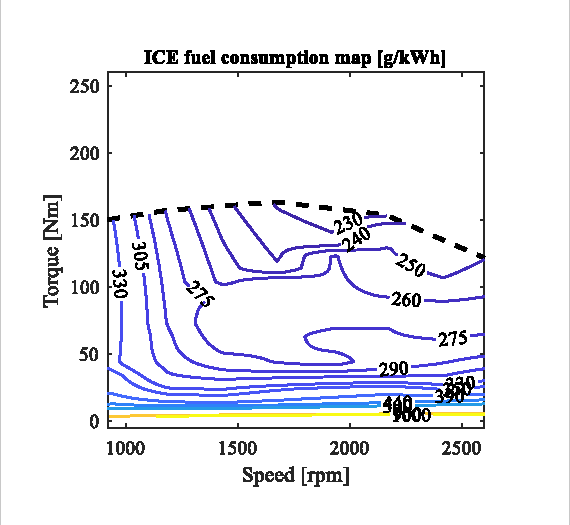
\includegraphics{ICE36.pdf} % Link to figure
        \caption{Sơ đồ khối của hệ thống} % figure name
        \label{hinh31}  % cross-reference for figure
    \end{figure}

Hình \ref{hinh31} là ví dụ về cách chèn ảnh. Lưu ý chú thích của hình vẽ được đặt ngay dưới hình vẽ. Tất cả các hình vẽ phải được đề cập đến trong phần nội dung và phải được phân tích và bình luận

\subsection{Cách tạo bảng}

    \begin{table}[H]
        \centering
        \caption{Kết quả thí nghiệm}
        \begin{tabularx}{0.85\textwidth}{
            | >{\centering}y%\arraybackslash}y
            | >{\centering\arraybackslash}a
            | >{\centering\arraybackslash}a
            | >{\centering\arraybackslash}y|
            }
                \hline
            \bfseries  Lần thí nghiệm   &\bfseries Điện áp đo được \hspace{1cm}(mV)   &\bfseries Điện áp tham chiếu \hspace{0pt} (mV)  & \bfseries Sai lệch\hspace{0pt}(\%)\\\hline
             1  &   &   &\\\hline
             2  &   &   &\\\hline
             3  &   &   &\\\hline
        ...  &   &   &\\\hline
        \end{tabularx}
            \label{bang31}
    \end{table}
    
Bảng \ref{bang31} là ví dụ về cách tạo bảng. Lưu ý chú thích của bảng được đặt ở trước bảng. Tất cả các bảng biểu phải được đề cập đến trong phần nội dung và phải được phân tích và bình luận.

\subsection{Viết phương trình}
    \begin{equation}\label{pt31}
        F(x) = \int^a_b \frac{1}{3}x^3
    \end{equation}
    
Phương trình \ref{pt31} là ví dụ về phương trình tích phân.

    \begin{equation}\label{pt32}
         x[t_n] = \frac{1}{\sqrt{N}} \sum_{k=0}^{N-1}X[f_k]e^{j 2\pi n k/N}
    \end{equation}
    
Phương trình \ref{pt32} thể hiện phép biến đổi Fourier rời rạc ngược (IDFT).

\newpage
%% --------------------------------------------------%%
%------------ CHAPTER 4 ---------------------------%
%%-----------------------------------------------------%
\section*{CHƯƠNG 4. MÔ PHỎNG VÀ KẾT QUẢ}
    \addcontentsline{toc}{section}{\numberline{} CHƯƠNG 4. MÔ PHỎNG VÀ KẾT QUẢ}
\setcounter{section}{4}
    \setcounter{figure}{0}
        \setcounter{table}{0}
            \setcounter{equation}{0}

%--------------------------------------------------------%

Các kết quả được thể hiện tại đây ...


\newpage

% CONCLUSIONS
\section*{KẾT LUẬN}
    \phantomsection\addcontentsline{toc}{section}{\numberline {}KẾT LUẬN}
    
Kết luận chung cho các chương trong đồ án.


\newpage

% REFERENCES
\phantomsection\addcontentsline{toc}{section}{\numberline {}TÀI LIỆU THAM KHẢO}

\bibliography{citation}
\newpage

% APPENDIX
\section*{PHỤ LỤC}
    \phantomsection\addcontentsline{toc}{section}{\numberline{} PHỤ LỤC}

Phụ lục cần thêm (nếu có)
...

\end{document}